\chapter{Elektromagnetiske Bølger}

I laserfysik stiftede I bekendtskab med lys som elektromagnetiske bølger, der består af et elektrisk- og magnetisk felt. Dette kapitel går i dybden med beskrivelsen af en elektromagnetisk bølge. Derudover vil kapitlet bruge denne til at beskrive polariseret lys, og hvordan lys opfører sig gennem optiske elementer. 

Kapitlet beskæftiger sig med matematik, der endnu ikke er præsenteret. I opfordres derfor til at læse A.4, A.5 og A.6 i appendikset. 

%og hvordan man kan bruge denne til at beskrive, hvordan lys opfører sig gennem optiske elementer samt hvordan det kan manipuleres.  

\section{Elektriske- og Magnetiske Felter}
I fysikken er felter et godt værktøj, og inden for elektrodynamik er de uundværlige. Vi vil især beskæftige os med vektorfelter, der er en funktion, der giver hvert punkt i rummet en tilhørende vektor. Et simpelt eksempel på et vektorfelt er tyngdeaccelerationen. Her peger $\zhat$ opad, så da feltet peger nedad er det negativt.
\begin{equation}
\v{g}(x,y,z) = -g\zhat
\end{equation}
Det elektriske felt kommer af Coulombs lov: $\v{F} = \frac{q_1q_2}{4\pi\varepsilon_0r^2}$, der beskriver kraften imellem to ladninger. Kraften på ladning 1 afhænger af begge ladninger. Kraftens størrelse afhænger af afstanden med en faktor $\frac{1}{r^2}$. $\frac{1}{4\pi\varepsilon_0}$, der er en konstant, i stil med $G$ i Newtons tyngdeligning, der minder meget om Coulombs lov. I fysik vil man gerne finde så gennerelle løsninger som muligt. Istedet for at finde kraften imellem de to ladninger finder man det elektriske felt $\v{E}$ fra hver ladning. Felterne er defineret så krafen på en ladning $q$ i feltet er 
\begin{equation}
\v{F}=\v{E}q.
\end{equation} 

Den magnetiske kraft på en ladning er lidt anderledes end den elektriske kraft, da den ikke kun afhænger af ladningen, men også hvor hurtigt og i hvilken retning ladningen bevæger sig. Man kan beskrive den magnetiske kraft ved magnetfeltet $\v{B}$ og ladningens hastighed $\v{v}$
\begin{equation}
\v{F} = q(\v{v}\times\v{B}).
\end{equation}
 

\section{Maxwells Ligninger}
Dannelsen af $\v E$-- og $\v B$--felterne beskrives af et sæt af fire ligninger, kaldet Maxwells ligninger. 
\begin{align}
\text{Gauss lov}~~~~~\v{\nabla}\cdot \v{E} &= \frac{\rho}{\varepsilon_0}\\
\text{"Gauss lov"\,for magnetisme}~~~~~\v{\nabla}\cdot \v{B} &= 0\\
\text{Faradays lov}~~~~~\v{\nabla}\times \v{E} &= -\frac{\partial \v{B}}{\partial t}\\
\text{Amperes lov}~~~~~\v{\nabla}\times \v{B} &= \mu_0\left(\varepsilon_0\frac{\partial \v{E}}{\partial t} + \v{j}\right)
\end{align}

Den første kaldes Gauss lov, og siger at $\v{E}$-felter udstråler fra elektriske ladninger. Her er $\rho$ tætheden af de elektriske ladninger, det vil sige ladningen per rumfang $\frac{q}{V}$. 
Den anden har ikke et officielt navn, men kaldes ofte Gauss lov for magnetisme, p.g.a. ligheden imellem de to. Den siger at der ikke findes magnetiske ladninger (monopoler).
Den tredje kaldes Faradays lov, og siger at en ændring i et $\v{B}$-felt skaber et $\v{E}$-felt.
Den sidste, kaldet Amperes lov, siger at en ændring i et $\v{E}$ felt giver et $\v{B}$-felt. Den siger også at man kan danne et $\v{B}$-felt med en elektrisk strøm. Her er $\v{j}$ strømtætheden, altså  strømstyrke per volumen. Bemærk, at strømstyrke normalt ses som en skalar, men da strømmen har både en størrelse og en retning, er det muligt at regne det som en vektor. Det er særligt interessant, når strømmen ikke er begrænset til at løbe i en ledning.

Derudover indgår to konstanter. $\varepsilon_0$ indgik også i Coulombs lov og hedder vakuumpermitiviteten, og er: $8,854\frac{\mathrm{C^2}}{\mathrm{N m}}$. 
Den anden konstant er $\mu_0$ og kaldes vakuum permeabiliteten. Den har størrelsen: $\mu_0 = 1,2566 \mathrm{\frac{N}{A^2}}$

Alt i elektrodynamik kan udledes fra disse fire love samt en femte, der beskriver, hvordan ladede partikler påvirkes af elektromagnetiske felter kaldet Lorentz kraften: $\v{F} = q(\v{E}+\v{v}\times\v{B})$.

\section{Bølgeligningen}
Figur \ref{fig:elektromagbolge} viser en elektromagnetisk bølge som den illustreres. Den består af et elektrisk-- og magnetisk felt, der svinger vinkelret på hinanden. Derudover er udbredelsesretningen givet som krydsproduktet af disse (prøv at overbevis dig selv om dette med højrehåndsreglen).
Men hvordan kan det være, at vi kan beskrive lys som denne bølge?
Først må \emph{bølgeligningen} introduceres. 


\begin{figure}[h!]
  \centering
  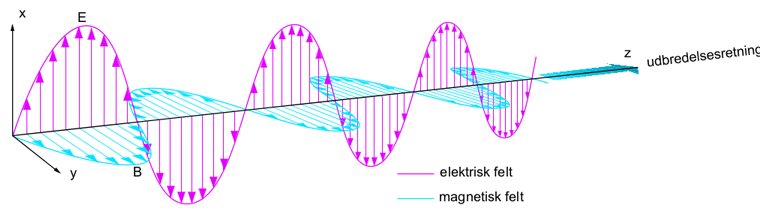
\includegraphics[width=\textwidth]{Elektrodynamik/EMbolge.png}
  \caption{Illustration af en elektromagnetisk bølge bestående af et elektrisk felt og et magnet felt, der svinger vinkelret på hinanden.}
  \label{fig:elektromagbolge}
\end{figure}

Grundlæggende set er en bølge en forstyrelse der udbreder sig, ofte i et medie. Det kan være krusningerne på overfladen af en dam, eller svingningerne i luften, vi opfanger som lyd. Mange fysiske fænomener beskrives som løsninger til anden--ordens--differentialligninger, bølger er ingen undtagelse. Ligningen bag bølgefænomener kaldes logisk nok for \emph{bølgeligningen}. I én dimension er den
\begin{equation}
\frac{\partial^2 f}{\partial z^2} = \frac{1}{v^2}\frac{\partial^2 f}{\partial t^2}
\label{eq:bolgeligning}
\end{equation}
hvor $v$ er bølgens hastighed. Det viser sig, at bølgeligningen kan løses af alle funktioner på formen: $f(x\pm vt)$ hvor $f$ er en vilkårlig funktion. Af særlig interesse er dog sinusbølger. De skrives dog ofte med cosinus:
\begin{equation}
f = A\cos\left(2\pi\left(\frac{z}{\lambda} - \nu t\right)+\phi\right) = A\cos\left( kz-\omega t+\phi\right)
\end{equation}
Her er $\lambda$ bølgelængden (afstanden imellem to bølgetoppe), $\nu$ (græsk $n$) er frekvensen (hvor mange toppe passerer et punkt over tid), som også kan skrives som $f$, $\phi$ er en forskydning af bølgen, og $k$ og $\omega$ kaldes bølgetallet og vinkelfrekvensen. De sidstnævnte spiller samme rolle som bølgelængden og frekvensen, men inkluderer $2\pi$. Sammenhængen mellem dem er: $$k=\frac{2\pi}{\lambda}~~ og ~~f = 2\pi\omega$$ For at opfylde bølgeligningen må der gælde at:
\begin{equation}
v = \nu\lambda = \frac{\omega}{k}
\end{equation}
\section{Elektromagnetiske Bølger}
Det antages, at den elektromagnetiske bølge udbreder sig i vakuum, hvorfor der hverken er ladninger eller elektriske strømme, så Maxwells ligninger forsimples en anelse. Det medfører at $\rho=0$ og $\v j=0$. 
\begin{align}
\text{Gauss lov}~~~~~\v{\nabla}\cdot \v{E} &= 0\\
\text{"Gauss lov"\,for magnetisme}~~~~~\v{\nabla}\cdot \v{B} &= 0\\
\text{Faradays lov}~~~~~\v{\nabla}\times \v{E} &= -\frac{\partial \v{B}}{\partial t}\\
\text{Amperes lov}~~~~~\v{\nabla}\times \v{B} &= \mu_0\varepsilon_0 \frac{\partial \v{E}}{\partial t}
\end{align}
Vi starter med at tage rotationen af $\v{E}$ to gange. Efter Faradays lov er  det:
\begin{equation}
\v{\nabla}\times (\v{\nabla}\times\v{E}) = -\v{\nabla}\times\frac{\partial \v{B}}{\partial t}
\end{equation}
Siden $\v{\nabla}\times$ og $\frac{\partial}{\partial t}$ differentierer med hensyn til forskellige variable, er deres rækkefølge underordnet. Det tillader os at indsætte Amperes lov på højre side:
\begin{equation}
\v{\nabla}\times (\v{\nabla}\times\v{E})  = -\frac{\partial}{\partial t}(\v{\nabla}\times \v{B}) = -\mu_0\varepsilon_0\frac{\partial^2 \v{E}}{\partial t^2}
\end{equation}
Vi er nu færdig med højre side, men venstre side kan gøres simplere. Dobbelt rotation viser sig at være: 
\begin{equation}
\v{\nabla}\times (\v{\nabla}\times\v{F}) =\v{\nabla}(\v{\nabla}\cdot \v{F})- \v{\nabla}^2\v{F} = \v{\nabla}(\v{\nabla}\cdot \v{F})-\frac{\partial^2 \v{F}}{\partial x^2}-\frac{\partial^2 \v{F}}{\partial y^2}-\frac{\partial^2 \v{F}}{\partial z^2}
\end{equation}
$\v \nabla(\v\nabla\cdot \v F)$ er gradienten af divergensen, $\v\nabla^2$ er endnu en operator kaldet vektor Laplace operatoren. Den findes ved at lægge den oprindelige vektor sammen dobbelt differentieret til hvert koordinat. 
Da $\v{\nabla}\cdot\v{E}=0$ findes differentialligningen:
\begin{equation}
\frac{\partial^2\v{E}}{\partial x^2}+\frac{\partial^2\v{E}}{\partial y^2}+\frac{\partial^2\v{E}}{\partial z^2} = \mu_0\varepsilon_0\frac{\partial^2 \v{E}}{\partial t^2}
\end{equation}
Dette er egentligt en bølgeligning, men vi kan reducere det til en en dimmesionel bølgeligning ved at antage, at $\v{E}$ altid ligger langs $x$ aksen.
\begin{equation}
\frac{\partial^2 \v{E}}{\partial x^2} = \mu_0\varepsilon_0\frac{\partial^2\v{E}}{\partial t^2}
\label{eq:Ebolgeligning}
\end{equation}
Der er intet særligt ved $x$-aksen, og $\v E$-feltet kunne lige så godt have enhver anden retning i $xy$-planen. $\v E$-feltet er dog altid vinkelret på udbredelsesretningen, så alt lys er transversale bølger. 

Sammenlignes ligning \ref{eq:bolgeligning} og \ref{eq:Ebolgeligning}, ses det at 
\begin{equation}
\frac{1}{v^2} = \mu_0\varepsilon_0 \Rightarrow v = \frac{1}{\sqrt{\mu_0\varepsilon_0}},
\end{equation}
og da denne bølge udbreder sig i vakuum, og lysets hastighed her i er $c$, må 
\begin{equation}
c = \frac{1}{\sqrt{\mu_0\varepsilon_0}}
\end{equation}
%Retningen af $\v E$-feltet angiver lystets polarisering. $\v E$-feltet fra polariseret lys kan skrives:
%\begin{equation}
%\v E = \begin{pmatrix}
%E_x\cos(kx-\omega t)\\
%E_y\cos(kx-\omega t)\\
%0
%\end{pmatrix}=
%\begin{pmatrix}
%E_x\\E_y\\0
%\end{pmatrix}
%\cos(kx-\omega t)
%\end{equation}
%Her ligger al informationen om lystets polarisering i vektoren, så hvis man arbejder med polariseret lys bruges ofte Jones vektorer. Det er en to dimmensionel vektor med $x$ og $y$ komposanterne.
%\begin{table}[h]
%\center
%\begin{tabular}{c|c r r}
%Polarisering &$\v E$-felt & Jones vektor & polariseringsvinkel\\\hline
%Vandret & $E_x\cos(kx-\omega t)\hat{\v x}$ & $\dbinom{1}{0}$&$0^\circ$\\
%Lodret & $E_y\cos(kx-\omega t)\hat{\v y}$ & $\dbinom{0}{1}$&$90^\circ$\\
%Diagonalt & $\dfrac{E}{\sqrt{2}}\cos(kx-\omega t)(\hat{\v x}+\hat{\v y})$ & $\tfrac{1}{\sqrt{2}}\dbinom{1}{1}$&$45^\circ$\\
%anitdiagonalt & $\dfrac{E}{\sqrt{2}}\cos(kx-\omega t)(\hat{\v x}-\hat{\v y})$ & $\tfrac{1}{\sqrt{2}}\dbinom{1}{-1}$&$-45^\circ$\\
%\end{tabular}
%\caption{Forskellige polariseringer og deres Jones vektorer}
%\end{table}

\section{Polariseret Lys}


Nu hvor I har set, at lys er elektromagnetiske bølger, og videre at disse bølger er transversale, kan vi kigge nærmere på, hvad polariseret lys er. Først vil vi dog kigge på begrebet polarisering, og hvad det egentligt betyder.\\

Polarisering er en egenskab, som alle transversale bølger har, og man kan derfor kigge på et simpelt eksempel, der illustrer begrebet. Tager man en snor og spænder den ud langs $z$--aksen, kan man lave en transversal bølge ved at tage fat i snorens ene ende, og svinge den op og ned langs $x$--aksen eller frem og tilbage langs $y$--aksen, som det er vist på Figur \ref{pol_lys}. I det første tilfælde vil udsvinget (forskydningen af snoren fra $z$-aksen) udelukkede ske langs $x$-aksen, og man siger, at bølgen er lineært polariseret\footnote{Grunden til at man kalder det "lineært polariseret" og ikke bare "polariseret" skyldes, at der findes andre former for polarisering. Vi vil dog ikke arbejde med disse andre former her, så hvis vi skriver, at noget er polariseret eller taler om polarisering, er det underforstået, at der menes lineært polariseret eller lineær polarisering.} i $x$-retningen (lodret). I det andet tilfælde vil udsvinget kun være langs $y$-aksen, og denne bølge er altså lineært polariseret i $y$-retningen (vandret). Man kunne selvfølgeligt også have svunget snoren skråt frem og tilbage imellem $x$- og $y$-aksen eller på en hvilken som helst anden led i $xy$-planen. Også i disse tilfælde, er det retningen af udsvinget, der bestemmer polariseringretningen. \\  

\begin{figure}[h!]
	\centering
	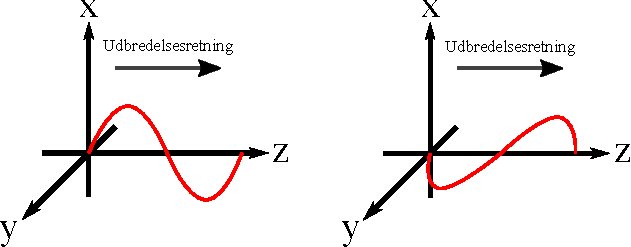
\includegraphics[scale=1.1]{Elektrodynamik/pol_lys_fig.pdf}
	\caption{Til venstre ses en transversalbølge på snoren, indikeret med rødt, hvor udsvinget er langs $x$-aksen. Til højre ses også en transversalbølge på snoren, hvor udsvinget er langs $y$-aksen. Endeligt er udbredelsesretningen, dvs. den retning som bølgen bevæger sig i, også indikeret.}
	\label{pol_lys}
\end{figure}


Polariseret lys, i sin simpleste form, er lys, der består af en enkelt elektromagnetisk bølge. Vi vil udelukkende arbejde med denne form, og derfor undersøge, hvordan man beskriver polariseringen af sådanne bølger. Da en elektromagnetisk bølge består både at et elektrisk felt, $\v{E}$, og et magnetisk felt, $\v{B}$, kan man definere polariseringen af bølgen, både ud fra den retning hvor $\v{E}$ har sit udsving, og den retning hvor $\v{B}$ har sit udsving. Det er dog kun nødvendigt at bruge en af disse, da både $\v{E}$- og $\v{B}$-feltet i en elektromagnetisk bølge er vinkelret på hinanden og på bølgens udbredelsesretning. Hvis man kender udbredelsesretningen og retningen af udsvinget for det ene felt, kan man også finde retningen af udsvinget for det andet. I fysikken er der tradition for, at man definerer polariseringen ud fra det elektriske felt, så det gør vi også her.\\

Det elektriske felt, for en elektromagnetiske bølge der udbreder sig langs $z$-aksen, kan skrives:

\begin{equation}
\v{E} = \xyz{E_x \cos \left( kz - \omega t \right)}{E_y \cos \left( kz - \omega t \right)}{0} = \xyz{E_x}{E_y}{0} \cos \left( kz - \omega t \right)
\label{Efelt_rigtige}
\end{equation}

\vspace{2mm}

Bemærk her, at $\v{E}$-feltets $z$-komposant altid er nul, når bølgens udbredelsesretning er langs $z$-aksen (husk at $\v{E}$-feltet er vinkelret på udbredelsesretningen). Da polariseringen af en enhver transversalbølge kun afhænger af, i hvilken retning udsvinget foregår, behøver man kun kigge på $x$ og $y$ komposanterne af $\v{E}$ fra (\ref{Efelt_rigtige}), for at beskrive bølgens polarisering. Videre er størrelsen, $\cos \left( kz - \omega t \right)$, som er det led, der får det elektriske felt til at svinge, ikke af nogen betydning ift. til den retning, som udsvinget har. Denne retning er udelukkende bestemt af tallene $E_x$ og $E_y$. Når man arbejder med polarisering af elektromagnetiske bølger, som udbreder sig langs $z$-aksen, skriver man det elektriske felt, $\v{E}$, som en 2-dimensional vektor\footnote{Alt der er gennemgået i vektorafsnittet i appendikset gælder også for vektorer i to dimensioner, med krydsproduktet som en enkelt undtagelse. Krydsproduktet er kun defineret for vektorer i tre dimensioner. Den første indgang i en 2D-vektor er stadig $x$-komposanten og den anden indgang er stadig $y$-komposanten.}

\begin{equation}
\kraft{\v{E}}{pol} = \xy{E_x}{E_y}
\label{Pol_Efelt} \ ,
\end{equation} 

\vspace{2mm}

hvor subscriptet "pol" er for at kende forskel på det rigtige $\v{E}$-felt, (\ref{Efelt_rigtige}), og den simplere version, (\ref{Pol_Efelt}), der bruges til at beskrive polariseringen. For at drage en parallel til eksemplet med snoren, kan man kigge på de to tilfælde, hvor enten $E_x$ eller $E_y$ er lig med nul\footnote{I to dimensioner har enhedsvektorene ikke nogen $z$-komposant og skrives: $\xhat = \begin{bsmallmatrix} 1 \\ 0 \\ \end{bsmallmatrix}$ og $\yhat = \begin{bsmallmatrix} 0 \\ 1 \\ \end{bsmallmatrix}$.}:

$$E_y = 0 \quad \Rightarrow \quad \kraft{\v{E}}{pol} = \xy{E_x}{0} = E_x \xhat \quad \quad \quad \text{og} \quad \quad \quad E_x = 0 \quad \Rightarrow \quad \kraft{\v{E}}{pol} = \xy{0}{E_y} = E_y \yhat$$

\vspace{2mm}

I det første tilfælde ($E_y = 0$) peger $\kraft{\v{E}}{pol}$ kun i $x$-retningen og repræsenterer en elektromagnetisk bølge, der er lineært polariseret i denne retning. På samme måde repræsenterer det andet tilfælde ($E_x=0$) en bølge, der er polariseret i $y$-retningen. Hvis både $E_x$ og $E_y$ er forskellige fra nul, kan man beskrive polariseringsretningen vha. den vinkel $\theta$, kaldet polariseringsvinklen, som $\kraft{\v{E}}{pol}$ laver med $x$-aksen (se Figur \ref{Efelt_pol}). Da skrives $\kraft{\v{E}}{pol}$ som

\begin{equation}
\kraft{\v{E}}{pol} = \xy{E_x}{E_y}   = | \kraft{\v{E}}{pol} | \xy{\cos \theta}{\sin \theta} \ ,
\label{E_pol}
\end{equation}

\vspace{2mm}

hvor det er brugt, at $E_x = | \kraft{\v{E}}{pol} | \cos \theta$, og at $E_y = | \kraft{\v{E}}{pol} | \sin \theta$. Dette og de to ovenstående tilfælde er illustreret på Figur \ref{Efelt_pol}. Bemærk også, at tilfældende $E_y = 0$ og $E_x = 0$ hhv. er specialtilfælde af (\ref{E_pol}), hvor $\theta$ er lig $0$ og $90$ grader.\\

\begin{figure}[h!]
	\centering
	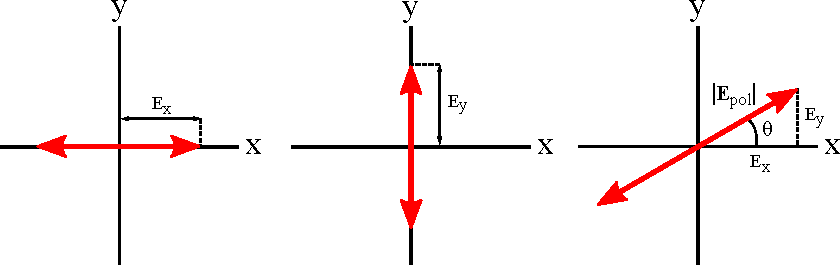
\includegraphics[scale=1]{Elektrodynamik/Efelt_pol_fig.pdf}
	\caption{Tre eksempler på et lineært polariseret $\v{E}$-felt. Polariseringsretningen er angivet med rødt, og pilene i enderne minder os om, at det rigtige $\v{E}$-felt, (\ref{Efelt_rigtige}), svinger frem og tilbage langs polariseringsretningen, når tiden går.}
	\label{Efelt_pol}
\end{figure}

Endeligt er der en sidste ting, man gør, for ydeligere at simplificere beskrivelsen af polariseringen. Det er at sætte $| \kraft{\v{E}}{pol} | = 1$, så $\kraft{\v{E}}{pol}$ bliver en enhedsvektor:

\begin{equation}
\kraft{\hatvec{E}}{pol} = \xy{\cos \theta}{\sin \theta}
\end{equation}

\vspace{2mm}

Vektorer af denne form, som bruges til beskrivelse af polariseringen, kaldes for \emph{Jones Vektorer}, og indeholder alt den information man skal bruge, for at undersøge og arbejde med, hvordan polariseret lys opfører sig. Der er vist nogle eksempler på $\v{E}$-felter (for elektromagnetiske bølger der udbreder sig langs $z$-aksen), og deres Jones vektorer i Tabel \ref{jones_tabel}\footnote{Husk at det rigtige $\v{E}$-felt er i tre dimensioner. Enhedsvektorene i kolonnen med $\v{E}$-felterne, er altså 3D-vektorer.}.\\

\renewcommand{\arraystretch}{2.8}
\setlength{\tabcolsep}{9pt}
\begin{table}[h!]
	\centering
	\begin{tabular}{c | c | c | c |}
		Polarisering &$\v E$-felt & Jones vektor & Polariseringsvinkel\\\hline
		Vandret & $E_x\cos(kz-\omega t)\hat{\v x}$ & $\begin{bsmallmatrix} 1 \\ 0 \\ \end{bsmallmatrix}$&$0^\circ$\\
		Lodret & $E_y\cos(kz-\omega t)\hat{\v y}$ & $\begin{bsmallmatrix} 0 \\ 1 \\ \end{bsmallmatrix}$&$90^\circ$\\
		Diagonalt & $\dfrac{\abs{\v{E}}}{\sqrt{2}}\cos(kz-\omega t)(\hat{\v x}+\hat{\v y})$ & $\frac{1}{\sqrt{2}} \begin{bsmallmatrix} 1 \\ 1 \\ \end{bsmallmatrix}$&$45^\circ$\\
		Antidiagonalt & $\dfrac{\abs{\v{E}}}{\sqrt{2}}\cos(kz-\omega t)(\hat{\v x}-\hat{\v y})$ & $\frac{1}{\sqrt{2}} \begin{bsmallmatrix} 1 \\ -1 \\ \end{bsmallmatrix}$&$-45^\circ$\\
		Generelt & $\abs{\v{E}}\cos(kz-\omega t)\left( \cos \theta \hat{\v x}+\sin \theta\hat{\v y} \right)$ & $\begin{bsmallmatrix} \cos \theta \\ \sin \theta\\ \end{bsmallmatrix}$  & $\theta$\\
	\end{tabular}
	\caption{Forskellige polariseringer og deres Jones vektorer.}
	\label{jones_tabel}
\end{table}

\renewcommand{\arraystretch}{1}
\setlength{\tabcolsep}{6pt}

\section{Polariseringselementer}

I det forrige afsnit blev polariseret lys introduceret, og vi kom frem til, at det kan beskrives vha. Jones vektorer. I dette afsnit skal vi kigge på, hvordan man laver polariseret lys ud fra ikke--polariseret lys, som er den mest almindelige type, man finder i naturen. Vi skal også kigge på nogle enkelte polariseringselementer, der er et vigtigt redskab, når man vil manipulere polariseret lys.\\

Ikke--polariseret lys består af mere end én elektromagnetisk bølge (oftest et meget højt antal), og typisk vil hver af disse have vidt forskellige polariseringsretninger. Skematisk kan man angive ikke--polariseret lys, som det ses på Figur \ref{ikke_pol_lys}. For at lave polariseret lys ud fra ikke--polariseret lys, må man finde en måde at sortere alle de polariseringsretninger fra, som man ikke er interesserede i. Dette bringer os til det første polariseringselement, kaldet et \emph{Lineært Polariseringsfilter}.\\

\begin{figure}[h!]
	\centering
	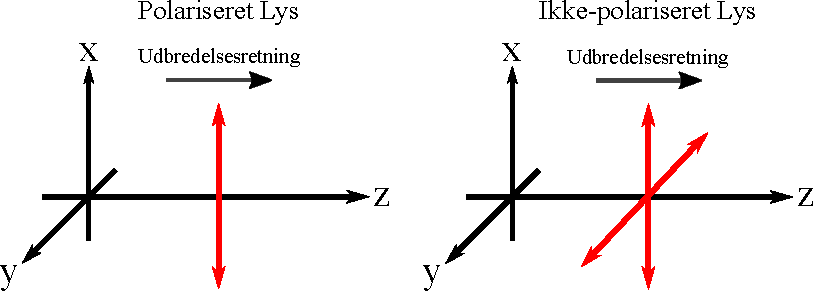
\includegraphics[scale=0.9]{Elektrodynamik/ikke_pol_lys.pdf}
	\caption{Til venstre ses en skematisk repræsentation af polariseret lys, der udbreder sig i $z$-retningen, og som er polariseret i $x$-retningen. Til højre ses en repræsentation af ikke-polariseret lys, hvilket er indikeret med en ekstra polariseringsretning.}
	\label{ikke_pol_lys}
\end{figure} 

Et lineært polariseringsfilter kan konstrueres på forskellige måder, men ideen er altid den samme. Polariseringsfilteret har en speciel akse, kaldet transmissionsaksen (TA), og det er kun elektromagnetiske bølger, hvis polarisering er sammenfaldende med denne akse, der kan passere igennem filteret. Et lineært polariseringsfilter fjerner altså alle de bølger i lyset, som ikke er polariserede langs TA, og efterlader kun en enkelt elektromagnetisk bølge, der er polariseret langs TA. Dette kan igen præsenteres skematisk, som det ses på Figur \ref{to_pol_filt}. Vi vil her ikke gå i dybden med, hvordan et lineært polariseringsfilter fjerner de elektromagnetiske bølger, der er polariseret forskelligt fra TA, men i stedet kigge nærmere på et andet polariseringselement, kaldet en \emph{Rotator}.\\

En rotator, som navnet indikerer, tager elektromagnetiske bølger med en give polarisering, og roterer polariseringsretningen omkring den aksen, hvor bølgen udbreder sig. Hvis en elektromagnetisk bølge med en polariseringsvinkel $\theta$ passerer igennem en rotator, vil den komme ud på den anden side, med en ny polariseringsvinkel $\theta + \beta$, hvor størrelsen af vinklen $\beta$ afhænger af den specifikke rotator. Her henvises til Figur \ref{to_pol_filt} for en skematisk præsentation af en rotator. Vi vil heller ikke her gå i dybden med den bagvedliggende mekanisme for en rotator, men vil i stedet bruge resten af afsnittet på at undersøge, hvordan et lineært polariseringsfilter og en rotator kan beskrives matematiks vha. $2 \times 2$ matricer kaldet \emph{Jones Matricer}. Det vil vi gøre ved at kigge på nærmere på produktet af $2 \times 2$ matricer og Jones vektorer.\\

\begin{figure}[h!]
	\centering
	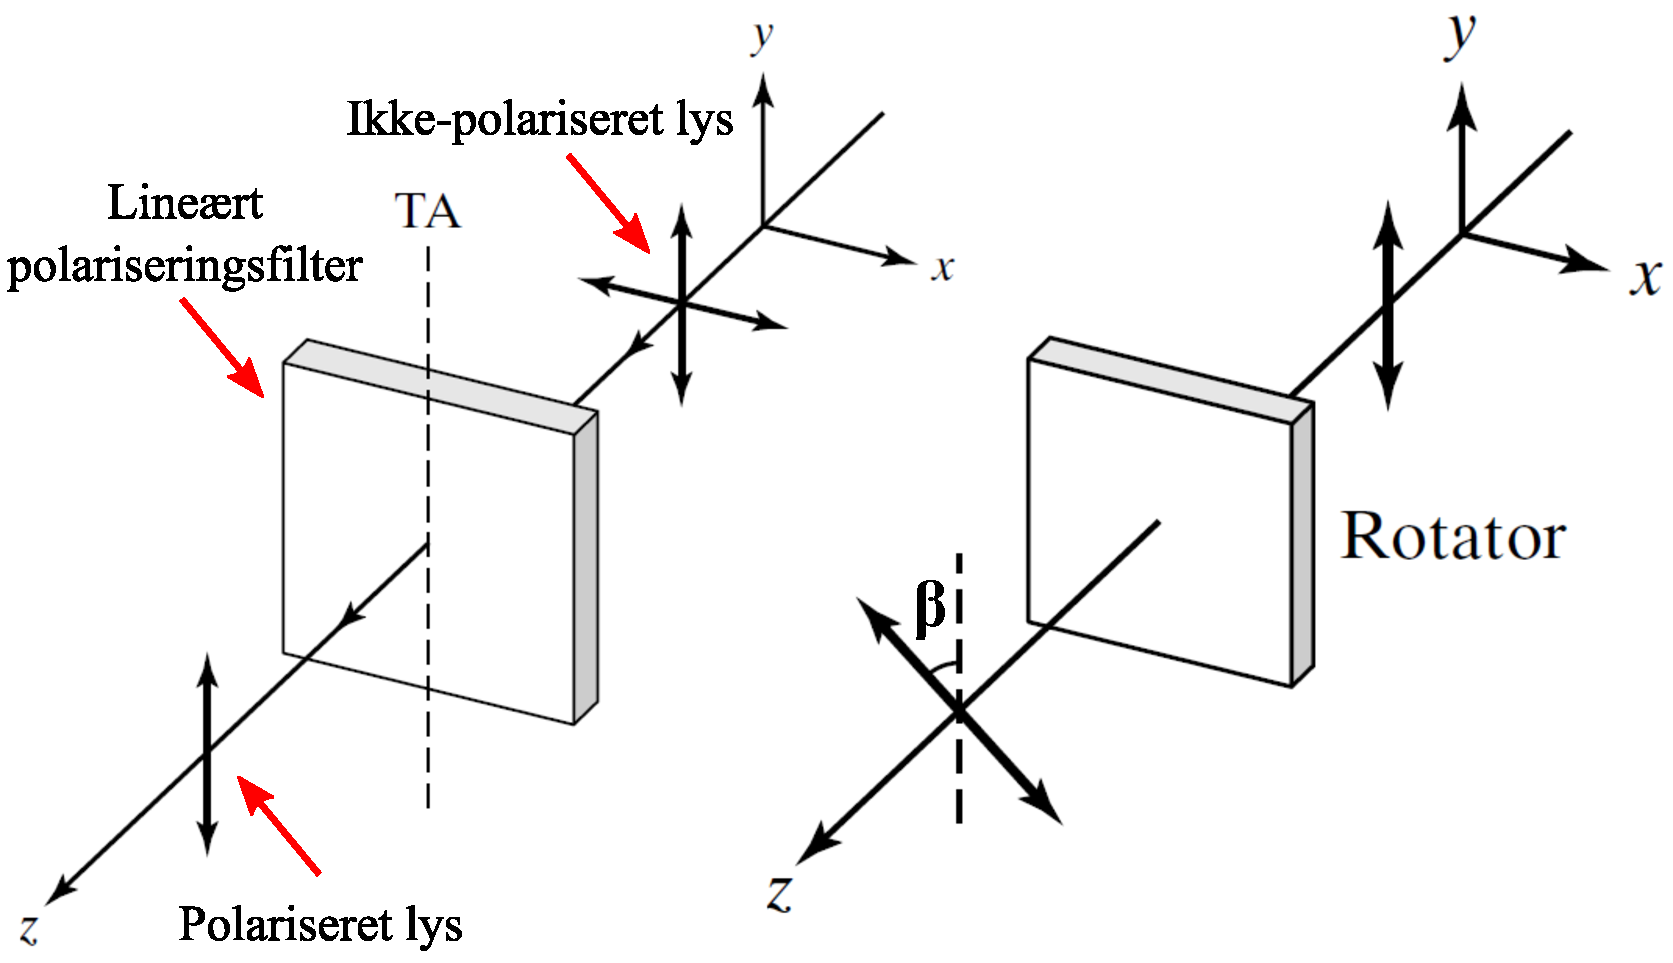
\includegraphics[scale=0.43]{Elektrodynamik/to_pol_filt.pdf}
	\caption{Skematisk præsentation af et lineært polariseringsfilter (til venstre) og en rotator (til højre).}
	\label{to_pol_filt}
\end{figure}

Den første Jones matrix, der undersøges, er for et lineært polariseringsfilter, hvor TA er langs $x$-aksen. Da vi endnu ikke ved, hvordan matricen skal se ud, skriver vi den op som en generel $2 \times 2$ matrix:

$$\v{M} =  \begin{bmatrix}
a & b \\ 
c & d \\
\end{bmatrix}$$ 

\vspace{2mm}

Da denne matrix skal repræsentere et filter med TA langs $x$-aksen, skal den ikke ændre Jones vektoren for en elektromagnetiske bølge polariseret i $x$-retningen, men den skal ændre Jones vektoren for en bølge polariseret i $y$-retningen (da denne bølge ikke kan passere igennem filteret, skal resultatet være nulvektoren). Denne viden giver os mulighed for at bestemme hvert af tallene $a,b,c,d$, ved at kigge på produktet af matricen med Jones vektorerne for disse typer af polariserede bølger:

$$\begin{bmatrix} a & b \\ c & d \\ \end{bmatrix} \xy{1}{0} = \xy{a \cdot 1 + b \cdot 0}{c \cdot 1 + d \cdot 0} = \xy{a}{c} = \xy{1}{0}$$

\vspace{2mm}

$$\begin{bmatrix} a & b \\ c & d \\ \end{bmatrix} \xy{0}{1} = \xy{a \cdot 0 + b \cdot 1}{c \cdot 0 + d \cdot 1} = \xy{b}{d} = \xy{0}{0}$$

\vspace{2mm}

I begge udtryk er produktet regnet ud (første lighedstegn), simplificeret (andet lighedstegn) og derefter sat lig med den Jones vektor (tredje lighedstegn), der repræsenterer den polariserede bølge efter det lineære polariseringsfilter. Man finder, at $a=1$ og $b=c=d = 0$. Jones matricen har da formen:

\begin{equation}
\v{M} = \begin{bmatrix} 1 & 0 \\ 0 & 0 \end{bmatrix} \quad \text{Lineært polariseringsfilter, TA langs $x$-aksen.}
\label{pol_filt_x}
\end{equation}

\vspace{2mm}

På samme måde kan man kigge på et lineært polariseringsfilter med TA langs $y$-aksen. Her vil Jones vektoren for en bølge polariseret i $y$-retningen ikke ændres, men Jones vektoren for en bølge polariseret i $x$-retningen bliver til nulvektoren. Bruger man samme metode som ovenfor, findes Jones matricen for dette filter til at være:

\begin{equation}
\v{M} = \begin{bmatrix} 0 & 0 \\ 0 & 1 \end{bmatrix} \quad \text{Lineært polariseringsfilter, TA langs $y$-aksen.}
\label{pol_filt_y}
\end{equation} 

\vspace{2mm}

For at kigge lidt nærmere på, hvordan en elektromagnetiske bølge ændrer sig, når den bevæger sig igennem et lineært polariseringsfilter, kan man kigge på eksemplet, hvor den generelle Jones vektor for en polariseringsvinkel $\theta$ (se Tabel \ref{jones_tabel}) passerer igennem et filter med TA langs $x$-aksen. Med de redskaber vi nu har, kan det skrives:

$$\begin{bmatrix} 1 & 0 \\ 0 & 0 \\ \end{bmatrix} \xy{\cos \theta}{\sin \theta} = \xy{1 \cdot \cos \theta + 0 \cdot \sin \theta}{0 \cdot \cos \theta + 0 \cdot \sin \theta} =  \xy{\cos \theta}{0}$$

\vspace{2mm}

Der er to ting at bemærke ved den resulterende vektor. For det første kan man se, at filteret kun fjerner den del af vektoren, som er vinkelret på TA (her er det $y$-komposanten), mens den del der er parallel med TA (her er det $x$-komposanten) ikke ændres. Dette er et generelt resultat, og gælder uanset hvordan TA og polariseringen af bølgen måtte være orienteret ift. hinanden. For det andet er længden af den resulterende vektor, $\sqrt{\cos^2 \theta + 0^2} = \sqrt{\cos^2 \theta}$, mindre end en, hvis $\theta \neq 0^\circ  ,  180^\circ$. Det skal fortolkes på den måde, at hvis polariseringen ikke er parallel med TA, så vil den elektromagnetiske bølge efter filteret, ikke bære lige så meget energi, som bølgen før filteret.\\



Den naturlige generalisering af resultaterne (\ref{pol_filt_x}) og (\ref{pol_filt_y}), er at finde Jones matricen for et lineært polariseringsfilter, hvor TA laver en vinkel $\alpha$ med den positive del af $x$-aksen. Det gøres igen ved at kigge på produktet mellem en general matrix og to forskellige Jones vektorer. Her vælges generelle Jones vektorer; en med samme vinkel $\alpha$ som TA, og en med vinkel $\alpha + 90^\circ$. Man får at:

$$\begin{bmatrix} a & b \\ c & d \\ \end{bmatrix} \xy{\cos \alpha}{\sin \alpha} = \xy{a \cos \alpha + b \sin \alpha}{c \cos \alpha + d \sin \alpha} = \xy{\cos \alpha}{\sin \alpha}$$

\vspace{2mm}

$$\begin{bmatrix} a & b \\ c & d \\ \end{bmatrix} \xy{\cos (\alpha + 90^\circ) }{\sin (\alpha + 90^\circ)} = \xy{a \cos (\alpha + 90^\circ) + b \sin (\alpha + 90^\circ)}{c \cos (\alpha + 90^\circ) + d \sin (\alpha + 90^\circ)} = \xy{0}{0}$$

\vspace{2mm}

Dette giver os fire ligninger med fire ubekendte:

\begin{align*}
a \cos \alpha + b \sin \alpha = \cos \alpha \quad \quad & \quad \quad c \cos \alpha + d \sin \alpha = \sin \alpha\\
\\
a \cos (\alpha + 90^\circ) + b \sin (\alpha + 90^\circ) = 0 \quad \quad & \quad \quad c \cos (\alpha + 90^\circ) + d \sin (\alpha + 90^\circ) = 0  
\end{align*}

\vspace{2mm}

Løses dette ligningssystem findes det, at $a = \cos^2 \alpha$, $b = c = \cos \alpha \sin \alpha$ og $d = \sin^2 \alpha$. Jones matricen er da:

\begin{equation}
\v{M} = \begin{bmatrix}
\cos^2 \alpha & \cos \alpha \sin \alpha\\
\cos \alpha \sin \alpha & \sin^2 \alpha \\
\end{bmatrix}
\quad \text{Lineært polariseringsfilter, TA vinkel $\alpha$.}
\end{equation}

\vspace{2mm}

Bemærk at tilfældende (\ref{pol_filt_x}) og (\ref{pol_filt_y}) er specialtilfælde af dette generelle resultat.\\

Vi vil nu kigge på, hvordan Jones matricen for en rotator ser ud. Som nævnt tidligere, skal en rotator tage en elektromagnetisk bølge med en polariseringsvinkel $\theta$ og ændre polariseringsvinklen til $\theta + \beta$. Denne gang behøver man kun kigge på produktet mellem en general matrix og en enkelt Jones vektor. Igen bruges den generelle Jones vektor, og man må kræve at:

$$\begin{bmatrix} a & b \\ c & d \\ \end{bmatrix} \xy{\cos \theta}{\sin \theta} = \xy{a \cos \theta + b \sin \theta}{c \cos \theta + d \sin \theta} = \xy{\cos (\theta + \beta)}{\sin (\theta + \beta)}$$

\vspace{2mm}

For at finde $a,b,c,d$ kan man bruge additionsformlerne for cosinus og sinus. Additionsformlerne er:
\begin{align*}
\cos (\theta + \beta) &= \cos \theta \cos \beta - \sin \theta \sin \beta\\
\\
\sin (\theta + \beta) &= \cos \theta \sin \beta + \sin \theta \cos \beta
\end{align*}

\vspace{2mm}

Ved sammenligning af additionsformlerne og udtrykket ovenfor, ses det, at $a = \cos \beta$, $b = - \sin \beta$, $c = \sin \beta$ og $d = \cos \beta$. Jones matricen for en rotator er da:

\begin{equation}
\v{M} = 
\begin{bmatrix}
\cos \beta & - \sin \beta \\
\sin \beta & \cos \beta \\
\end{bmatrix}
\quad \text{Rotator, vinkel $\beta$.} 
\end{equation}

Man kan nu spørge sig selv, om en rotator ændrer længden af en Jones vektor, som det var tilfældet med et lineært polariseringsfilter. Længden af en generel Jones vektor, som er ganget med Jones matricen for en rotator er:

$$\sqrt{\cos^2 (\theta + \beta) + \sin^2 (\theta + \beta)} = \sqrt{1} = 1$$

\vspace{2mm}

En rotator ændrer således ikke længden af den Jones vektor, som den ganges på, hvilket fortæller os, at en elektromagnetiske bølge, som passerer igennem en rotator, ikke mister noget af den energi, som bølgen bærer.\\

Til sidst skal det nævnes, at med de redskaber der er præsenteret i dette afsnit, kan man nu beskrive, hvad der sker med en elektromagnetisk bølge, hvis den passerer igennem et vilkårligt antal af lineære polariseringsfilter og rotatorer placeret i en række efter hinanden. Man tager Jones matricerne, for de polariseringselementer man bruger, kald dem $\v{M_1}, \v{M_2}, \v{M_3},\ldots,\v{M_n}$, hvor tallene angiver rækkefølgen, så $\v{M_1}$ er det polariseringselement bølgen passerer først, og ganger dem sammen\footnote{Når man ganger mere end to matricer sammen, har rækkefølgen betydning for resultatet. Det er derfor vigtigt at gange matricerne sammen i den rigtige rækkefølge! }:

\begin{equation}
\v{M_s} = \v{M_n} \v{M_{n-1} \cdots \v{M_3} \v{M_2} \v{M_1} }  
\end{equation}  

\vspace{2mm}

Så kan man tage den resulterende matrix, $\v{M_s}$, og gange på den Jones vektor, som repræsenterer den givne bølge.

